\chapter{Anforderungen \& Planung}

\section{Aufbau der Infrastruktur \& Technische Details}

Die Applikationen werden für das Betriebssystem Android in der Programmiersprache Java entwickelt, wobei auf API-Level 21 (Android 5.0) zurückgegriffen wird. Android Studio stellt dabei die Entwicklungsumgebung der Wahl dar. \\
Als Protokoll zum Austausch der Nachrichten wird das MQTT-Protokoll verwendet. Die zugrundeliegende MQTT-Software heißt \textit{Mosquitto}. \\
Die zentrale Serverkomponente \gf{Home Manager}, die für bestimmte Funktionen (siehe Abschnitt \ref{home_manager}) genutzt wird, wird ebenfalls in der Programmiersprache Java geschrieben. Dabei wird zum persistenten Speichern von Informationen die auf MySQL basierende Datenbank MariaDB verwendet. \\
Die Mikrocontroller, die für die Steuerung der LED-Lichterketten verantwortlich sind, basieren auf dem ESP8266 CPU. Der verwendete NodeMCU V3 koppelt diese Architektur mit einem WLAN-Chip und 13 GPIO Pins, wodurch der Mikrocontroller Nachrichten empfangen kann und Informationen für die Lichtsteuerung über GPIO Pins ausgeben kann. Das Programm auf diesen wird mithilfe der Arduino IDE in der Programmiersprache C geschrieben. \\ 
Die Infrastruktur ist in Abbildung \ref{fig:architecture} dargestellt. Die Android-Geräte mit den entsprechenden Apps werden im Folgenden als \textit{Sender} bezeichnet, da sie überwiegend Befehle zum Message-Broker senden. Dieser wertet die Nachrichten aus und stellt die den entsprechenden Empfängern zu. Die Nachrichten werden über das jeweilige Topic identifiziert, d.h. jede LED besitzt ein eigenes Topic, sodass jede LED einzeln angesteuert werden kann. Dabei folgen die Topics dem Schema \textit{Kanal/Zimmer/Gerät/Funktion}, sodass auch mehrere LED Streifen in einem Raum angesprochen werden können. Die Nachricht selbst enthält die Information, wie die LEDs leuchten sollen. Die Nachrichten werden von dem im WLAN-Netzwerk angemeldeten Mikrocontroller empfangen und verarbeitet. Diese im Folgenden als \textit{Empfänger} bezeichneten Geräte führen die gewünschte Aktion aus, bspw. das Leuchten der LED Steifen in den gewünschten Farben. \\
Für die Notation der Nachrichten wurde sich für JSON entschieden. 

\subsubsection*{Server-Komponente \textit{Home Manager}}
Die Nachricht wird außerdem noch vom sog. \textit{Home Manager} empfangen, der für sich relevante Nachrichten herausfiltert und verarbeitet. Zu seinen Funktionalitäten gehört die Umsetzung einer Timer-Funktion. In einer der beiden Apps soll eine Funktion eingebaut werden, um Timer einzustellen, d.h. dass zu bestimmten Uhrzeiten bestimmte LEDs automatisch angesteuert werden. So kann erreicht werden, dass man bspw. durch Hellwerden am Morgen geweckt wird oder abends das Licht bereits angeschaltet ist, wenn man nach Hause kommt. Dies soll durch Eintragungen der Zeitpunkte in die Datenbank MariaDB geschehen, welche in bestimmten Intervallen gelesen wird und die LEDs durch die HomeManager-Komponente aktiviert werden. Aufgrund der Komplexität und den Rahmenbedingungen dieser Arbeit im Rahmen des Moduls \gf{Mobile Applikationen} ist diese Funktion allerdings optional.


\begin{figure}
	\centering
	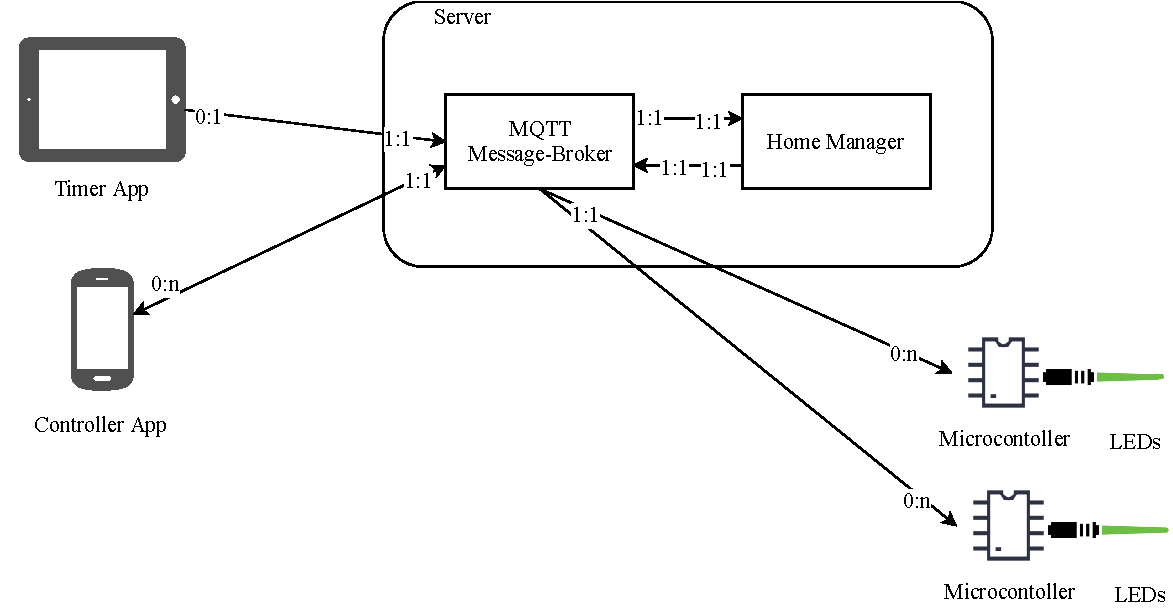
\includegraphics[width=\linewidth]{../images/architecture}
	\caption[Architektur der Smart-Home Infrastruktur]{Architektur der Smart-Home Infrastruktur}
	\label{fig:architecture}
\end{figure}


\section{Funktionale Anforderungen}

Die Infrastruktur der SmartHome-Anwendung soll dazu in der Lage sein, die folgenden Anwendungsfälle zu unterstützen:
\begin{itemize}
	\item Es ist möglich, sich mit jedem möglichen Gerät im Netzwerk (im Speziellen dem WLAN-Netzwerk) anzumelden und bestimmten Topics zuzuhören und Nachrichten zu diesen zu senden. So kann später auch eine Anwendung für Windows-PCs oder eine Webanwendung entwickelt werden. Diese Arbeit beschäftigt sich nur mit der Implementierung zweier Android-Apps als Frontend.
	\item Durch die Anmeldung der empfangenden Geräte, wie in dieser Arbeit die verwendeten LED-Lichterkette, kann prinzipiell jedes angemeldete Gerät angesteuert werden. Ein anderer denkbarer Ansatz wäre beispielsweise die Ansteuerung von Jalousinen über die beschriebene Infrastruktur.
	\item Die Server-Komponente auf dem Raspberry Pi übernimmt dabei besondere Aufgaben, die entweder zentral verwaltet werden müssen, wie bpsw. Timer-Funktionalität (siehe \ref{home_manager}), oder die nicht auf den Mikrocontrollern realisiert werden können (siehe \ref{impl_mikrocontroller}).
\end{itemize}

\section{Nicht-funktionale Anforderungen}

Neben den funktionalen Anforderungen müssen einige nicht-funktionale Anforderungen erfüllt werden, um die Erstellung und Weiterentwicklung der Lösung zu gewährleisten. Dazu zählen insbesondere
\begin{itemize}
	\item die Erstellung eines sauberen Programmcodes, sodass auch spätere Entwickler weiterhin am Projekt arbeiten können.
	\item die Performanz der Lösung, damit diese frustfrei verwendet werden kann.
	\item die Absturzsicherheit der verschiedenen Programme, sodass keine manuellen Neustarts oder dergleichen getätigt werden müssen. 
	\item die Übersichtlichkeit der Apps, damit der Nutzer diese möglichst intuitiv bedienen kann.
	\item die Skalierbarkeit, sodass spätere Komponenten möglichst einfach hinzugefügt werden können.
\end{itemize}



